\subsection{Example 1: A neuron-level MLP (tier L0)}\label{sec:ex01}
{\small set: official test \textbullet{} sample: \texttt{L0\_0803} \textbullet{} tier L0 \textbullet{} augmentation: \texttt{aug\_variant\_3} \textbullet{} topology seen in training \textbullet{} 10 nodes}

\lstinputlisting[style=py]{code/ex01.py}
\begin{center}\footnotesize\begin{tabular}{lcccccp{4.6cm}}\toprule
model & valid & edge F1 & exact & shape acc. & tokens & failure labels \\ \midrule
9B zero-shot & no & 0.55 & no & 0.88 & 268 & \raggedright naming only \tabularnewline
9B fine-tuned & yes & 1.00 & yes & 1.00 & 263 & \raggedright -- \tabularnewline
\bottomrule\end{tabular}\end{center}
\textbf{What to look at.} Every hidden unit is its own \texttt{Linear(k,1)} (``neurons'' made explicit). This
sample is an \emph{augmented} variant: the forward argument is renamed (\texttt{inp\_tensor}), a dead layer is inserted
and the \texttt{\_\_init\_\_} order is shuffled. The zero-shot 9B model wires the graph correctly (it is
\emph{isomorphic} to the reference) but names the input after the argument instead of \texttt{x}, picks the wrong input
width ($[1,3]$ instead of $[1,2]$) and therefore gets node and edge \emph{names} wrong: strict edge F1 is only 0.55
although the shape of the graph is right. The fine-tuned 9B reproduces the reference exactly.

\begin{figure}[H]\centering
\begin{minipage}[b]{0.32\linewidth}\centering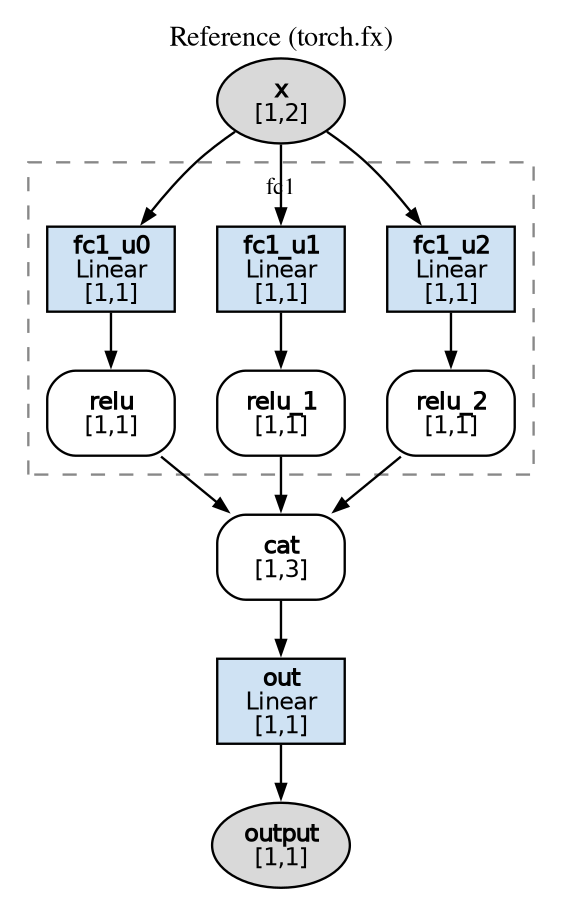
\includegraphics[width=\linewidth,height=0.40\textheight,keepaspectratio]{figs/ex01_ref.png}\\\footnotesize Reference\end{minipage}\hfill
\begin{minipage}[b]{0.32\linewidth}\centering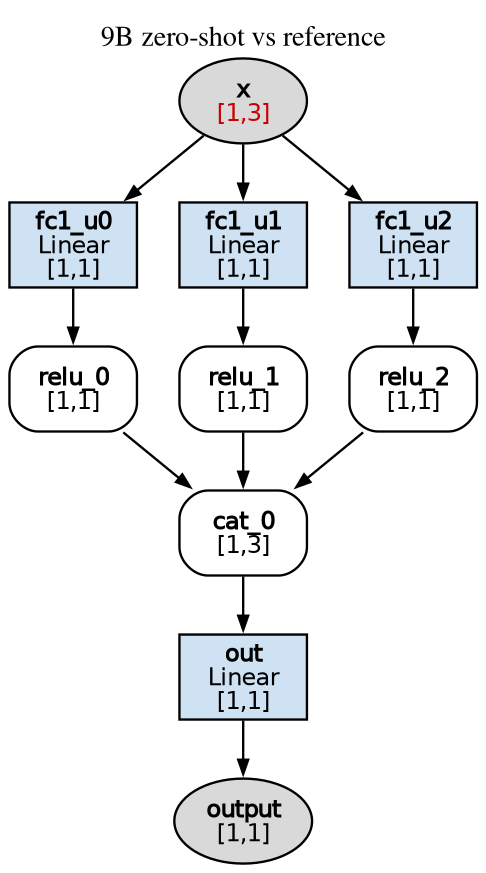
\includegraphics[width=\linewidth,height=0.40\textheight,keepaspectratio]{figs/ex01_base9b_zs_c_diff.png}\\\footnotesize 9B zero-shot vs reference\end{minipage}\hfill
\begin{minipage}[b]{0.32\linewidth}\centering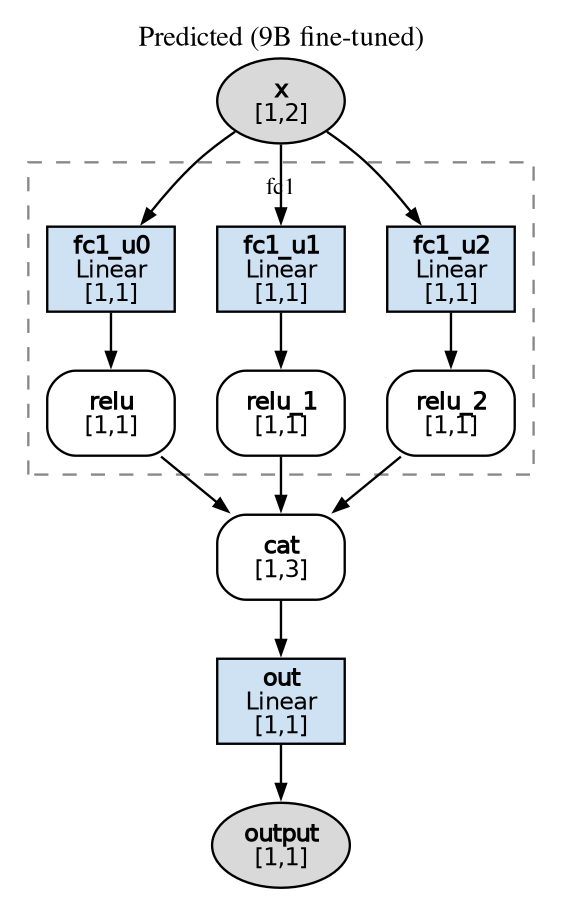
\includegraphics[width=\linewidth,height=0.40\textheight,keepaspectratio]{figs/ex01_ft9b_c_pred.png}\\\footnotesize 9B fine-tuned (exact)\end{minipage}\hfill
\caption{Example 1 (L0\_0803). Diff colours: black = matched, red dashed = missing (reference only), orange = hallucinated (prediction only), red text = wrong kind or shape.}
\end{figure}
\clearpage

\subsection{Example 2: A linear chain with dead code (tier L1)}\label{sec:ex02}
{\small set: official test \textbullet{} sample: \texttt{L1\_0886} \textbullet{} tier L1 \textbullet{} augmentation: \texttt{aug\_variant\_2} \textbullet{} topology seen in training \textbullet{} 6 nodes}

\lstinputlisting[style=py]{code/ex02.py}
\begin{center}\footnotesize\begin{tabular}{lcccccp{4.6cm}}\toprule
model & valid & edge F1 & exact & shape acc. & tokens & failure labels \\ \midrule
9B fine-tuned & yes & 1.00 & yes & 1.00 & 196 & \raggedright -- \tabularnewline
\bottomrule\end{tabular}\end{center}
\textbf{What to look at.} \texttt{self.unused\_op\_*} is declared and even \emph{called}, but its result never
reaches the \texttt{return}, so \texttt{torch.fx} (after dead-code elimination) does not contain it. The validator
checks exactly this (rule ``dead code included''). The fine-tuned model skips the dead call correctly. Over the whole test
set the base Coder-7B model included dead code in 34.6\% of the dead-code samples, the 9B 3-shot model in 0\%.

\begin{figure}[H]\centering
\begin{minipage}[b]{0.47\linewidth}\centering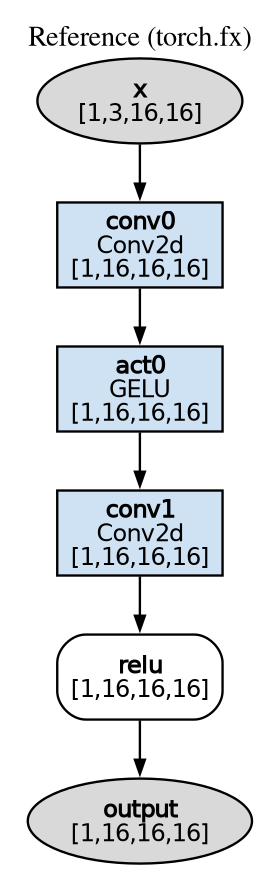
\includegraphics[width=\linewidth,height=0.40\textheight,keepaspectratio]{figs/ex02_ref.png}\\\footnotesize Reference (dead code removed)\end{minipage}\hfill
\begin{minipage}[b]{0.47\linewidth}\centering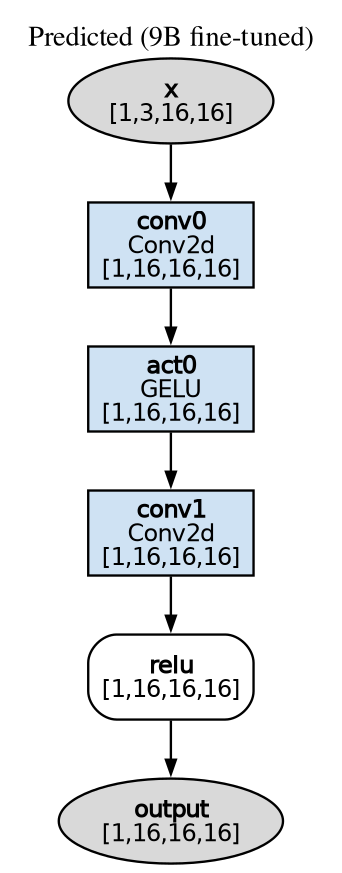
\includegraphics[width=\linewidth,height=0.40\textheight,keepaspectratio]{figs/ex02_ft9b_c_pred.png}\\\footnotesize 9B fine-tuned (exact)\end{minipage}\hfill
\caption{Example 2 (L1\_0886). Diff colours: black = matched, red dashed = missing (reference only), orange = hallucinated (prediction only), red text = wrong kind or shape.}
\end{figure}
\clearpage

\subsection{Example 3: A residual network (tier L2): the missing skip edge}\label{sec:ex03}
{\small set: official test \textbullet{} sample: \texttt{L2\_0804} \textbullet{} tier L2 \textbullet{} topology \textbf{held out} from training \textbullet{} 18 nodes}

\lstinputlisting[style=py]{code/ex03.py}
\begin{center}\footnotesize\begin{tabular}{lcccccp{4.6cm}}\toprule
model & valid & edge F1 & exact & shape acc. & tokens & failure labels \\ \midrule
9B 3-shot & no & 0.86 & no & 1.00 & 706 & \raggedright missing skip edge, missing edge, extra edge \tabularnewline
9B fine-tuned & yes & 1.00 & yes & 1.00 & 644 & \raggedright -- \tabularnewline
\bottomrule\end{tabular}\end{center}
\textbf{What to look at.} A residual network whose structure was \emph{held out} from fine-tuning. The 3-shot
base model gets every node right (node F1 1.0) but miswires the edges: the red dashed edges are reference edges it
missed (including the long \emph{skip connection} into an \texttt{add}), orange edges are ones it invented, and it emits
edges to node indices that do not exist (\texttt{edge [17, 18] points outside the 18 nodes}). Long-range skip edges
are the single most common failure of the prompted models (the \texttt{missing\_skip\_edge} label in Figure~\ref{fig:F7}).
The fine-tuned 9B gets this held-out topology exactly right.

\begin{figure}[H]\centering
\begin{minipage}[b]{0.47\linewidth}\centering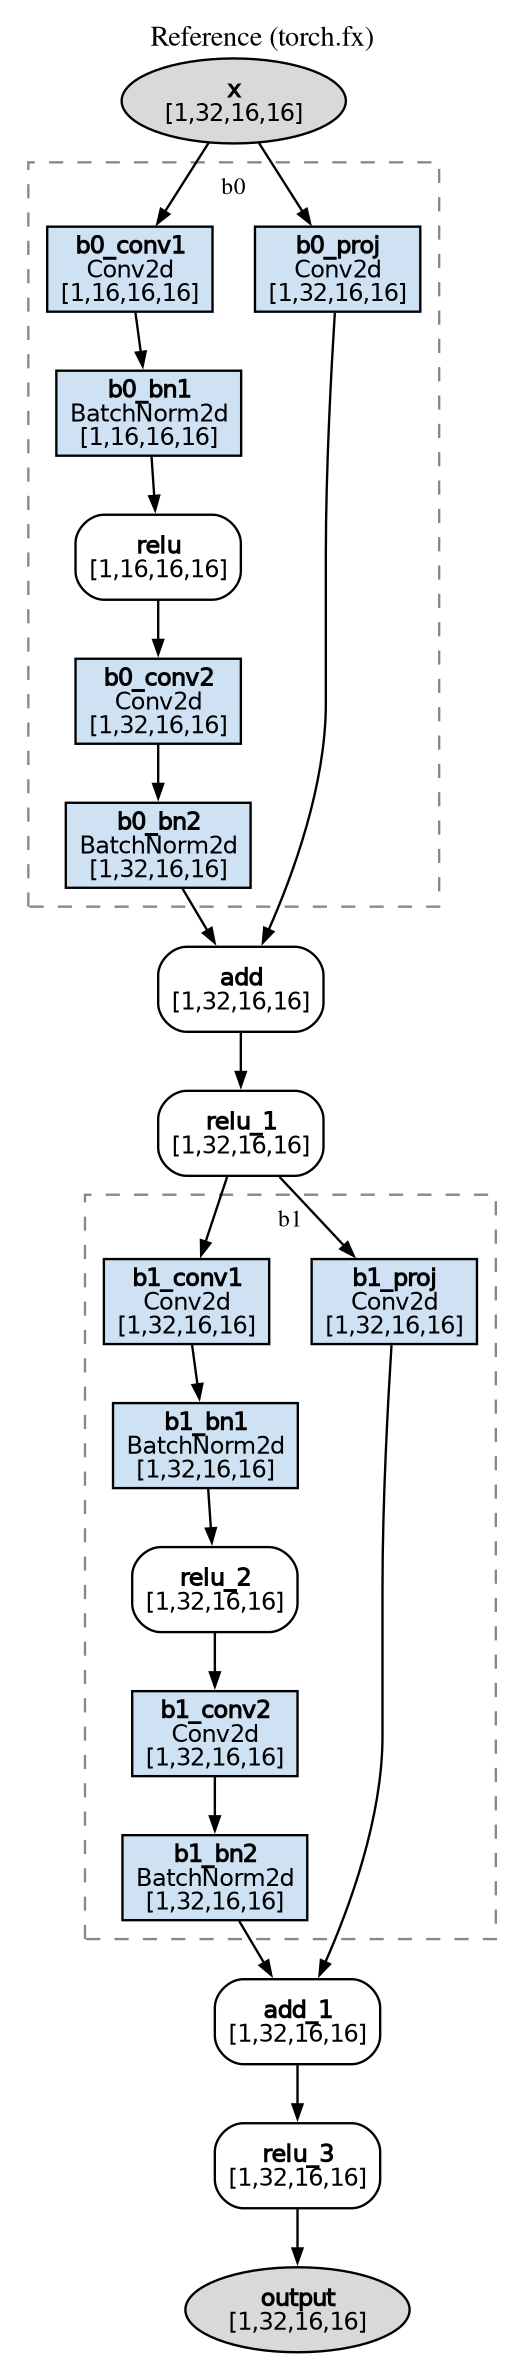
\includegraphics[width=\linewidth,height=0.40\textheight,keepaspectratio]{figs/ex03_ref.png}\\\footnotesize Reference\end{minipage}\hfill
\begin{minipage}[b]{0.47\linewidth}\centering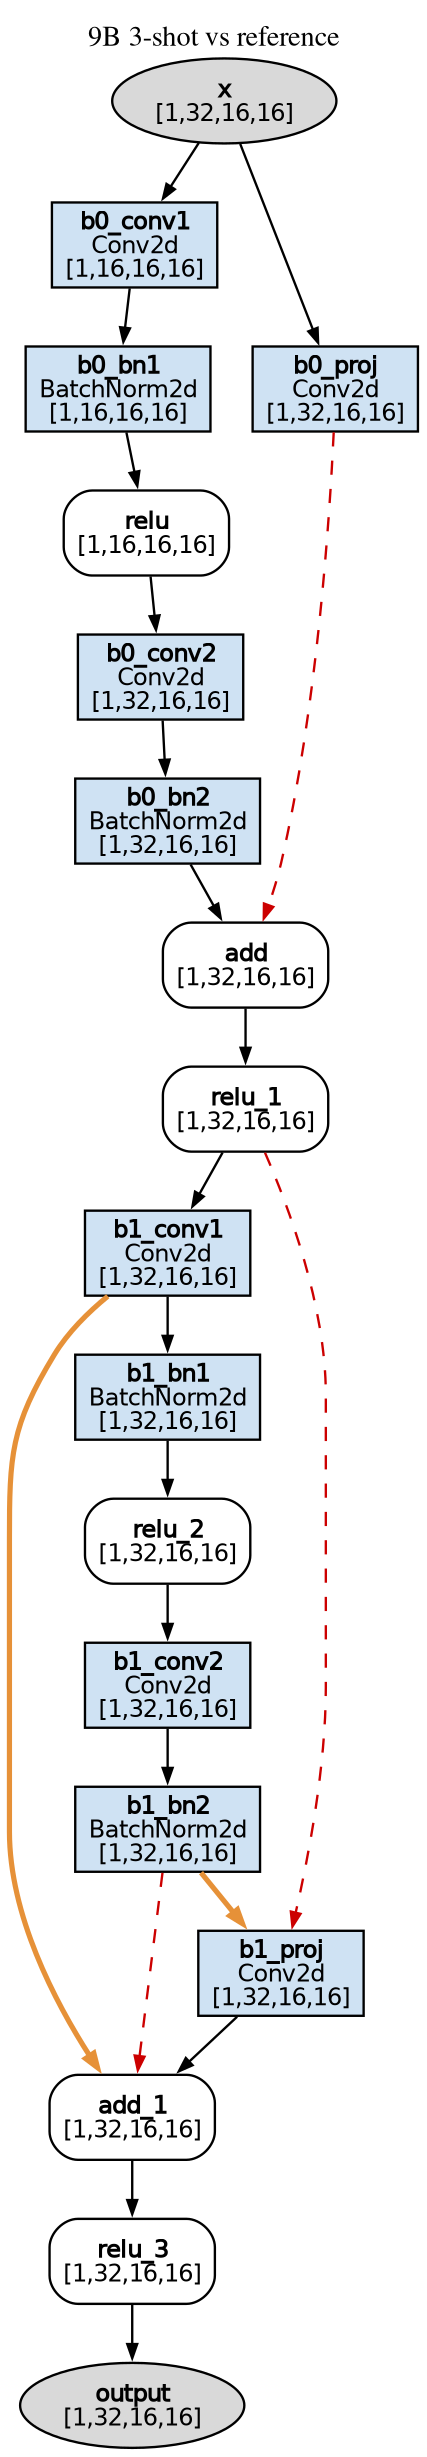
\includegraphics[width=\linewidth,height=0.40\textheight,keepaspectratio]{figs/ex03_base9b_fs_c_diff.png}\\\footnotesize 9B 3-shot vs reference\end{minipage}\hfill
\caption{Example 3 (L2\_0804). Diff colours: black = matched, red dashed = missing (reference only), orange = hallucinated (prediction only), red text = wrong kind or shape.}
\end{figure}
\clearpage

\subsection{Example 4: Parallel branches joined by concat (tier L3)}\label{sec:ex04}
{\small set: official test \textbullet{} sample: \texttt{L3\_0804} \textbullet{} tier L3 \textbullet{} topology seen in training \textbullet{} 12 nodes}

\lstinputlisting[style=py]{code/ex04.py}
\begin{center}\footnotesize\begin{tabular}{lcccccp{4.6cm}}\toprule
model & valid & edge F1 & exact & shape acc. & tokens & failure labels \\ \midrule
9B 3-shot & yes & 1.00 & yes & 1.00 & 405 & \raggedright -- \tabularnewline
\bottomrule\end{tabular}\end{center}
\textbf{What to look at.} Several parallel branches read the same tensor and are joined by
\texttt{torch.cat}. Branching and merging nodes are easy to spot in the drawing (out-degree $>1$, in-degree $>1$).
Here even the prompted 3-shot model is exactly right; tier L3 is the easiest multi-path tier for it (60.5\% exact).

\begin{figure}[H]\centering
\begin{minipage}[b]{0.47\linewidth}\centering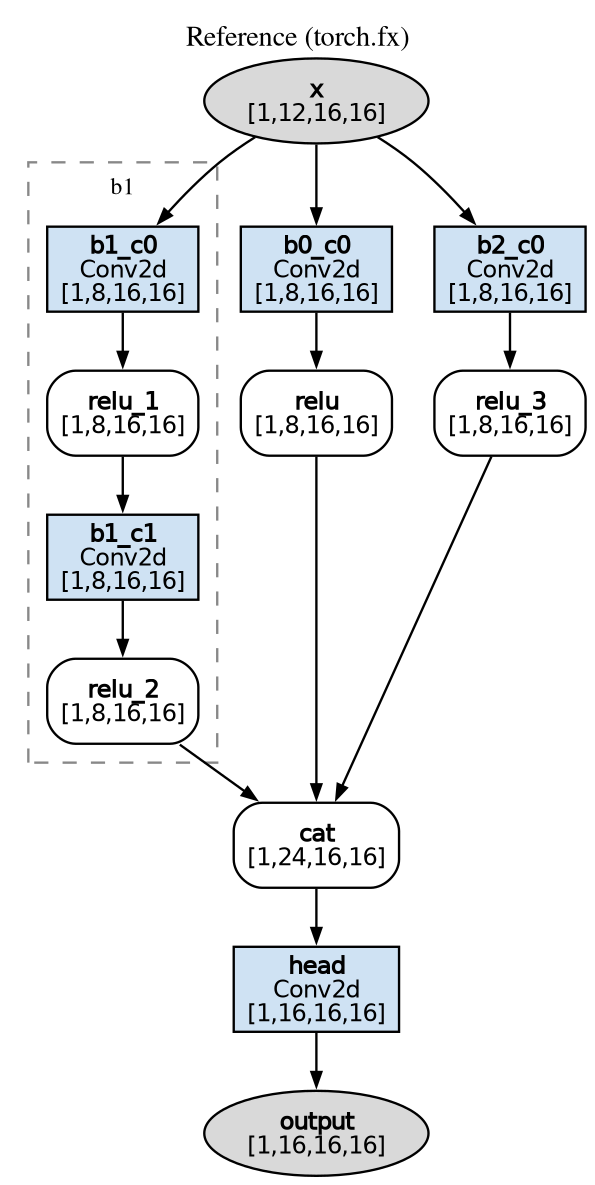
\includegraphics[width=\linewidth,height=0.40\textheight,keepaspectratio]{figs/ex04_ref.png}\\\footnotesize Reference\end{minipage}\hfill
\begin{minipage}[b]{0.47\linewidth}\centering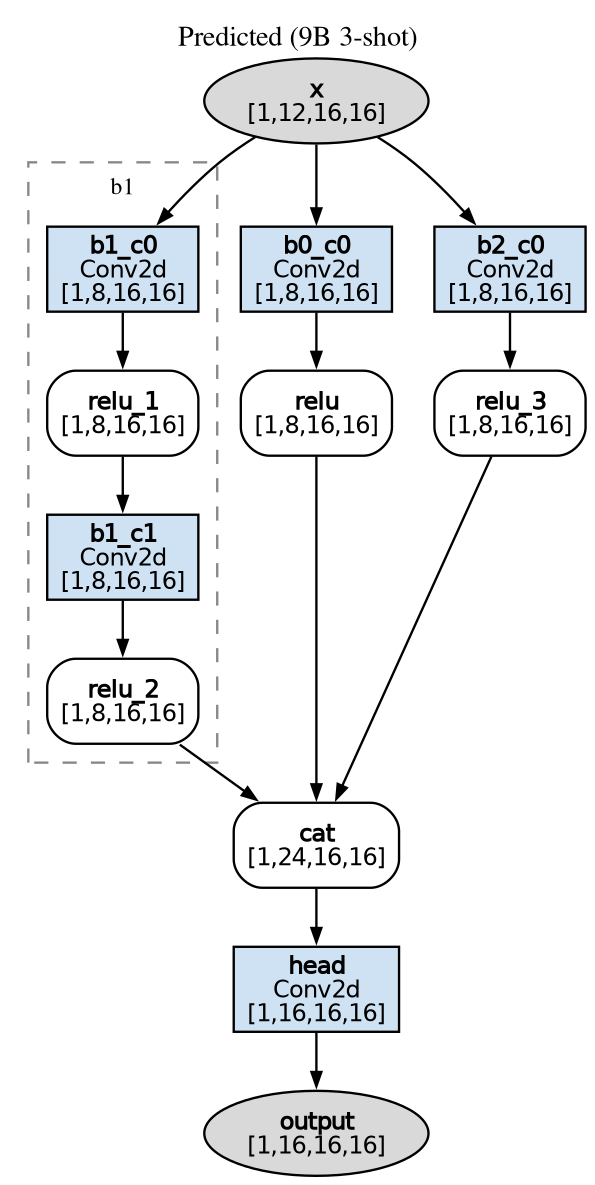
\includegraphics[width=\linewidth,height=0.40\textheight,keepaspectratio]{figs/ex04_base9b_fs_c_pred.png}\\\footnotesize 9B 3-shot (exact)\end{minipage}\hfill
\caption{Example 4 (L3\_0804). Diff colours: black = matched, red dashed = missing (reference only), orange = hallucinated (prediction only), red text = wrong kind or shape.}
\end{figure}
\clearpage

\subsection{Example 5: A held-out nested topology (tier L4): memorisation vs generalisation}\label{sec:ex05}
{\small set: official test \textbullet{} sample: \texttt{L4\_0800} \textbullet{} tier L4 \textbullet{} topology \textbf{held out} from training \textbullet{} 19 nodes}

\lstinputlisting[style=py]{code/ex05.py}
\begin{center}\footnotesize\begin{tabular}{lcccccp{4.6cm}}\toprule
model & valid & edge F1 & exact & shape acc. & tokens & failure labels \\ \midrule
2B fine-tuned & no & 0.92 & no & 1.00 & 638 & \raggedright missing skip edge, extra edge \tabularnewline
9B fine-tuned & yes & 1.00 & yes & 1.00 & 643 & \raggedright -- \tabularnewline
\bottomrule\end{tabular}\end{center}
\textbf{What to look at.} The nested L4 pattern (stem $\to$ two paths $\to$ concat $\to$ merge $\to$
residual add $\to$ head) with the one L4 structure that was held out of training. The fine-tuned \textbf{2B} writes
the nodes correctly but wires them like the L4 templates it saw in training: the validator reports
\texttt{'cat' has 1 input}, \texttt{'merge' has 2 inputs; a Conv2d takes exactly 1} and \texttt{'add' has 1 input
(missing skip edge?)}. All 52 held-out L4 test samples fail this way for the 2B (0\%), while the fine-tuned
\textbf{9B} gets 100\% of them. This is the clearest memorisation-vs-generalisation contrast in the project.

\begin{figure}[H]\centering
\begin{minipage}[b]{0.47\linewidth}\centering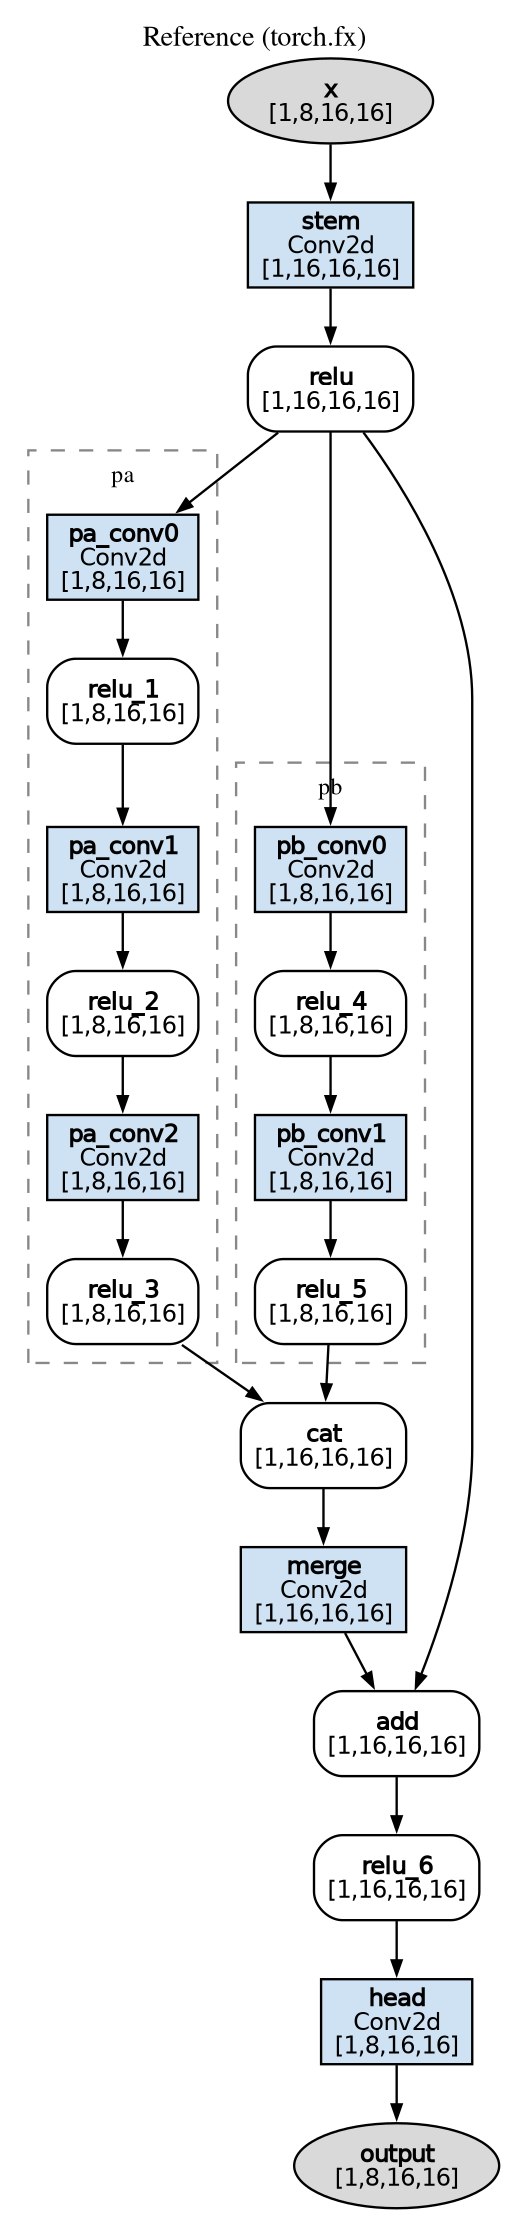
\includegraphics[width=\linewidth,height=0.40\textheight,keepaspectratio]{figs/ex05_ref.png}\\\footnotesize Reference\end{minipage}\hfill
\begin{minipage}[b]{0.47\linewidth}\centering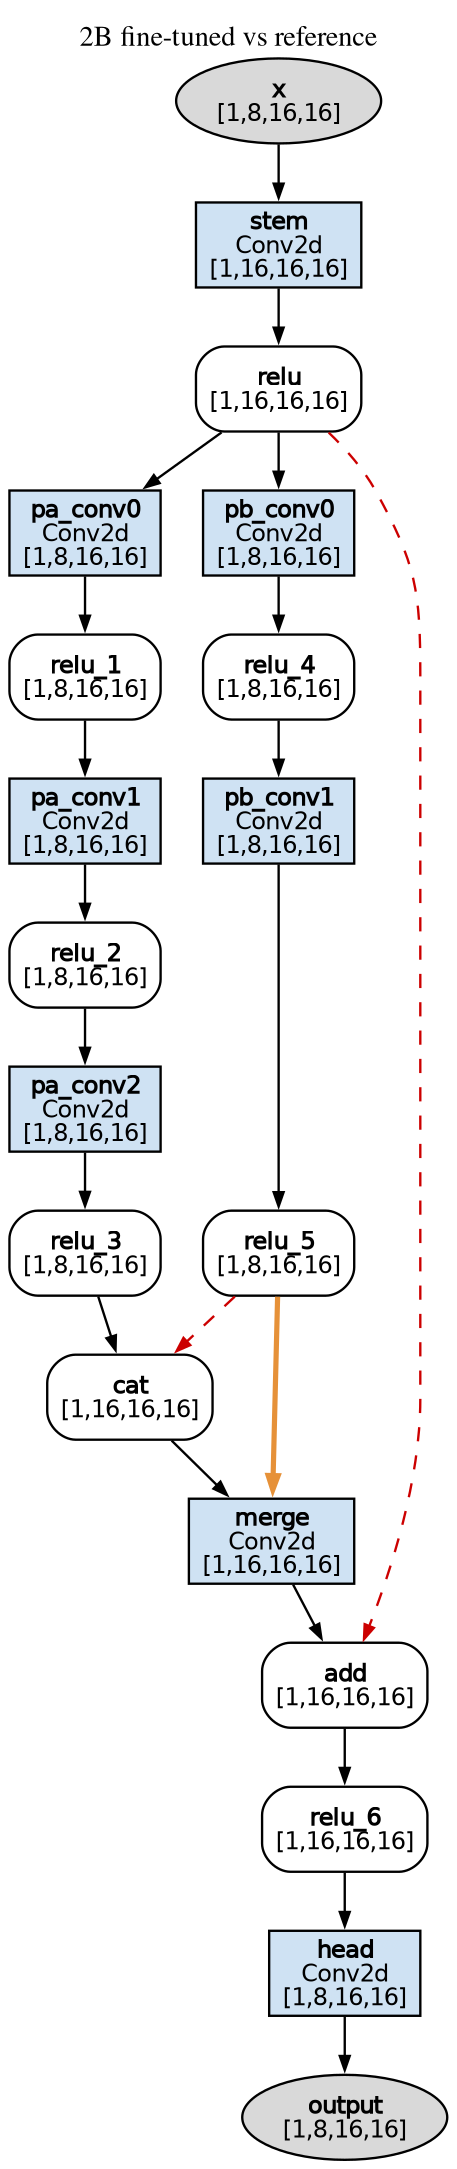
\includegraphics[width=\linewidth,height=0.40\textheight,keepaspectratio]{figs/ex05_ft2b_c_diff.png}\\\footnotesize 2B fine-tuned vs reference\end{minipage}\hfill
\caption{Example 5 (L4\_0800). Diff colours: black = matched, red dashed = missing (reference only), orange = hallucinated (prediction only), red text = wrong kind or shape.}
\end{figure}
\clearpage

\subsection{Example 6: The zero-shot runaway loop}\label{sec:ex06}
{\small set: official test \textbullet{} sample: \texttt{L0\_0857} \textbullet{} tier L0 \textbullet{} augmentation: \texttt{aug\_variant\_1} \textbullet{} topology seen in training \textbullet{} 14 nodes}

\lstinputlisting[style=py]{code/ex06.py}
\begin{center}\footnotesize\begin{tabular}{lcccccp{4.6cm}}\toprule
model & valid & edge F1 & exact & shape acc. & tokens & failure labels \\ \midrule
9B zero-shot & no & 0.00 & no & 0.00 & 3072 & \raggedright parse fail \tabularnewline
\bottomrule\end{tabular}\end{center}
\textbf{What to look at.} Nothing is wrong with the code; the failure is in decoding. The zero-shot 9B starts
a plausible answer, then falls into a loop in the edge list (\texttt{[n,n+1]} with ever larger \texttt{n}) until the
3{,}072-token limit stops it. The output is not a usable graph (parse/schema failure). 22\% of zero-shot test answers
ended like this (mostly on the larger L2/L4 graphs); fine-tuned models never did (Section~\ref{sec:journey}).

\begin{figure}[H]\centering
\begin{minipage}[b]{0.55\linewidth}\centering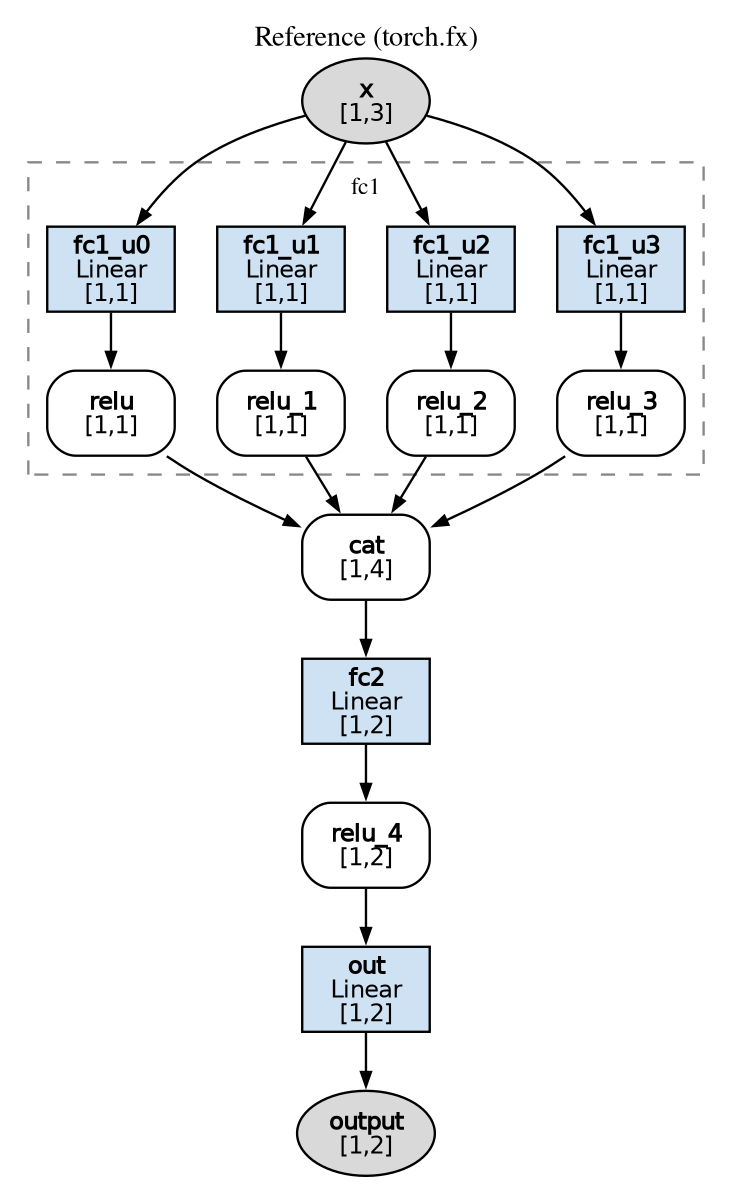
\includegraphics[width=\linewidth,height=0.36\textheight,keepaspectratio]{figs/ex06_ref.png}\\\footnotesize Reference\end{minipage}\hfill
\caption{Example 6 (L0\_0857). Diff colours: black = matched, red dashed = missing (reference only), orange = hallucinated (prediction only), red text = wrong kind or shape.}
\end{figure}
\noindent\textit{End of the zero-shot answer (cut off at 3{,}072 tokens):}
\begin{lstlisting}[style=plain]
..., 354], [354, 355], [355, 356], [356, 357], [357, 358], [358, 359], [359, 360], [360, 361], [361, 362], [362, 363], [363, 364], [364, 365], [365, 366], [366, 367], [367, 368], [368, 369], [369, 370], [370, 371], [371, 372], [372, 
\end{lstlisting}
\clearpage

\subsection{Example 7: OOD: nested submodules (dotted scopes)}\label{sec:ex07}
{\small set: OOD-1 \textbullet{} sample: \texttt{OOD\_resnet\_nested\_2} \textbullet{} category: \texttt{nested\_basicblock} \textbullet{} 13 nodes}

\lstinputlisting[style=py]{code/ex07.py}
\begin{center}\footnotesize\begin{tabular}{lcccccp{4.6cm}}\toprule
model & valid & edge F1 & exact & shape acc. & tokens & failure labels \\ \midrule
9B fine-tuned & no & 0.27 & no & 1.00 & 256 & \raggedright missing skip edge, missing edge, extra edge, missing node \tabularnewline
9B FT + synthetic & yes & 1.00 & yes & 1.00 & 435 & \raggedright -- \tabularnewline
\bottomrule\end{tabular}\end{center}
\textbf{What to look at.} An out-of-distribution module: a \emph{submodule class} \texttt{ResUnit} used twice.
\texttt{torch.fx} inlines nested modules and names their layers with the full path (\texttt{unit\_a\_conv\_a},
scope \texttt{unit\_a.conv\_a}). The dataset only has flat models, so the fine-tuned 9B writes \texttt{conv\_a} (a
name that is not declared at the top level: the validator flags it as possibly hallucinated) and collapses the two
units into one (the whole second unit is red dashed = missing). After adding synthetic training modules that contain
nested classes, the model gets it exactly right.

\begin{figure}[H]\centering
\begin{minipage}[b]{0.32\linewidth}\centering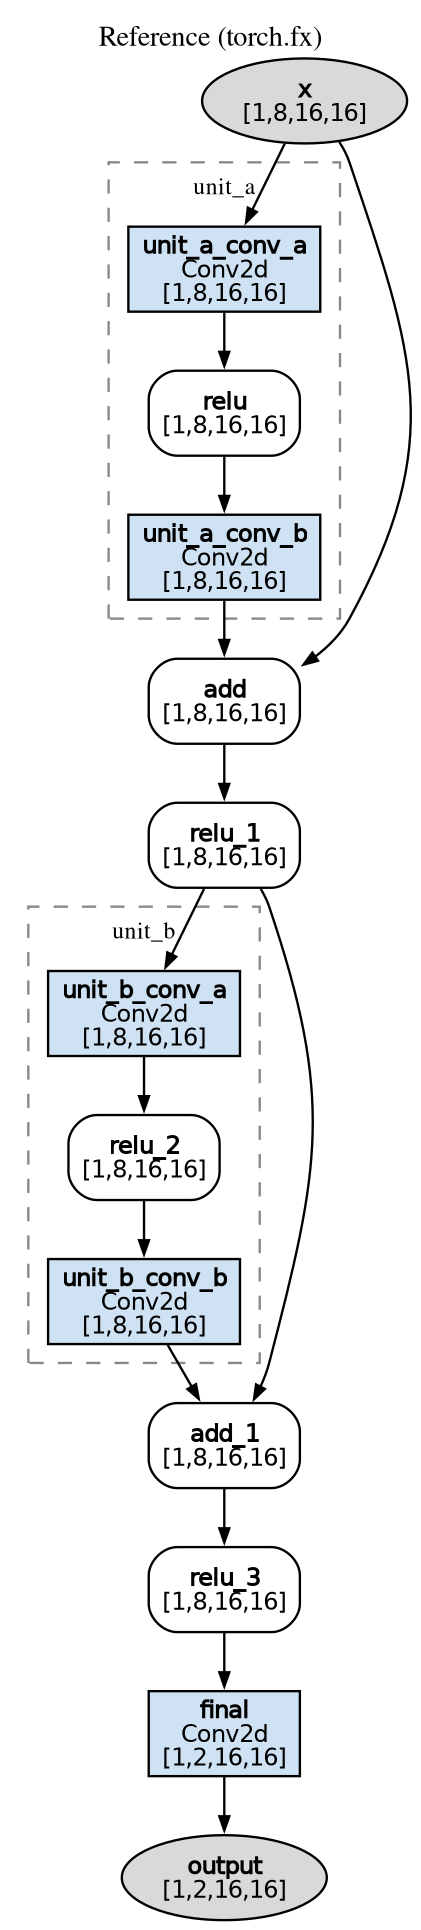
\includegraphics[width=\linewidth,height=0.40\textheight,keepaspectratio]{figs/ex07_ref.png}\\\footnotesize Reference\end{minipage}\hfill
\begin{minipage}[b]{0.32\linewidth}\centering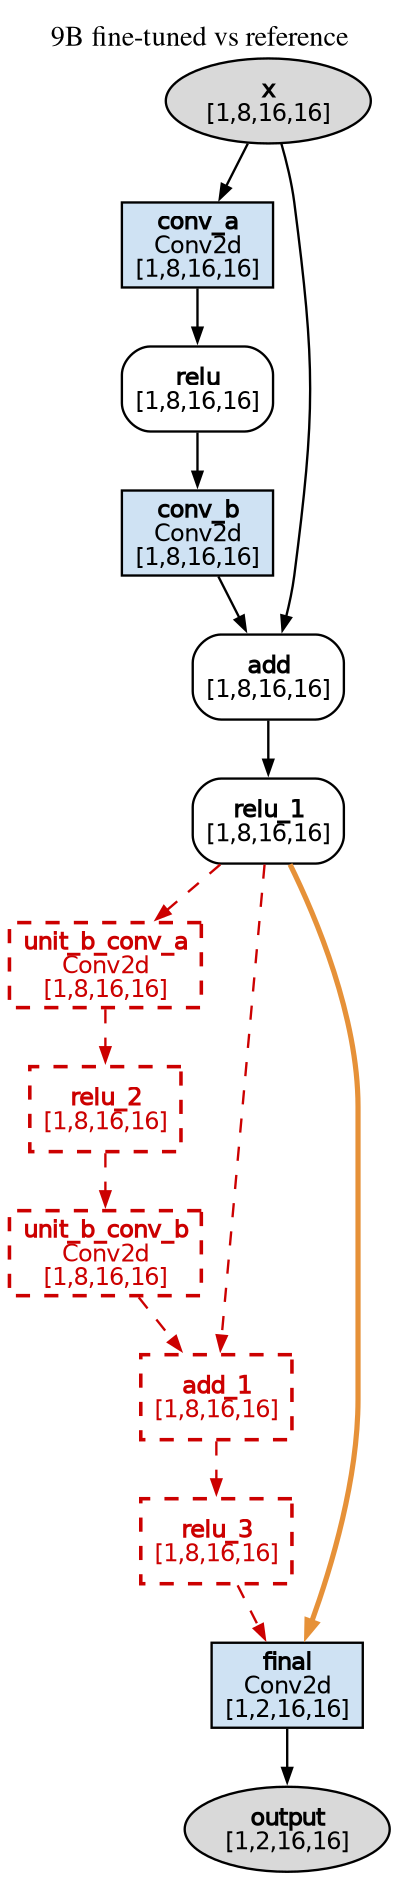
\includegraphics[width=\linewidth,height=0.40\textheight,keepaspectratio]{figs/ex07_ft9b_c_diff.png}\\\footnotesize 9B fine-tuned vs reference\end{minipage}\hfill
\begin{minipage}[b]{0.32\linewidth}\centering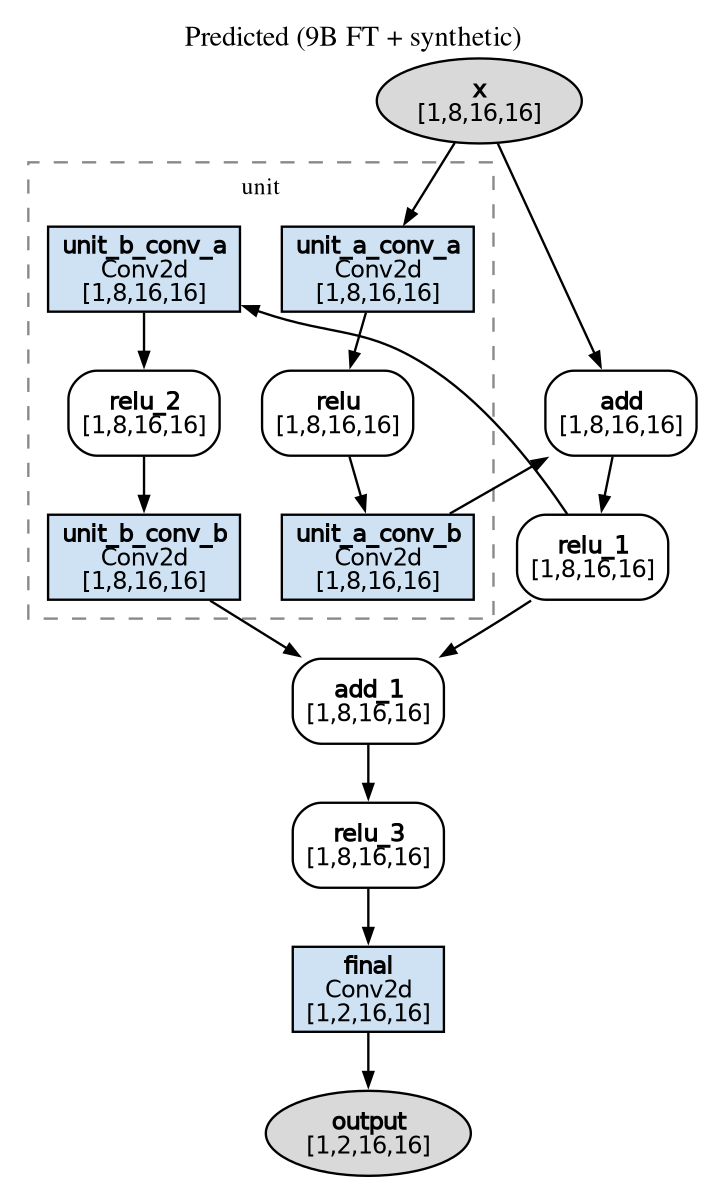
\includegraphics[width=\linewidth,height=0.40\textheight,keepaspectratio]{figs/ex07_ft9b_aug_c_pred.png}\\\footnotesize 9B FT + synthetic (exact)\end{minipage}\hfill
\caption{Example 7 (OOD\_resnet\_nested\_2). Diff colours: black = matched, red dashed = missing (reference only), orange = hallucinated (prediction only), red text = wrong kind or shape.}
\end{figure}
\clearpage

\subsection{Example 8: OOD: an nn.ModuleList loop}\label{sec:ex08}
{\small set: OOD-1 \textbullet{} sample: \texttt{OOD\_modulelist\_1} \textbullet{} category: \texttt{modulelist} \textbullet{} 9 nodes}

\lstinputlisting[style=py]{code/ex08.py}
\begin{center}\footnotesize\begin{tabular}{lcccccp{4.6cm}}\toprule
model & valid & edge F1 & exact & shape acc. & tokens & failure labels \\ \midrule
9B fine-tuned & no & 0.75 & no & 1.00 & 226 & \raggedright naming only \tabularnewline
9B FT + synthetic & yes & 1.00 & yes & 1.00 & 228 & \raggedright -- \tabularnewline
\bottomrule\end{tabular}\end{center}
\textbf{What to look at.} \texttt{nn.ModuleList} plus a Python \texttt{for} loop: \texttt{torch.fx}
unrolls the loop and names the layers \texttt{layers\_0}, \texttt{layers\_1}, \texttt{layers\_2}. The fine-tuned 9B
draws the right structure (isomorphic) but names the nodes \texttt{layers}, \texttt{layers\_1}, \dots, so strict
metrics and the code-consistency check fail (``naming only'' failure). The synthetic-data model names them correctly.

\begin{figure}[H]\centering
\begin{minipage}[b]{0.32\linewidth}\centering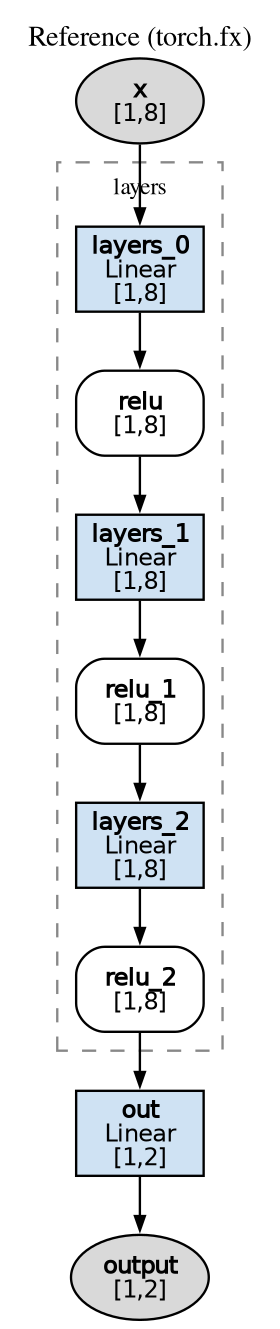
\includegraphics[width=\linewidth,height=0.40\textheight,keepaspectratio]{figs/ex08_ref.png}\\\footnotesize Reference\end{minipage}\hfill
\begin{minipage}[b]{0.32\linewidth}\centering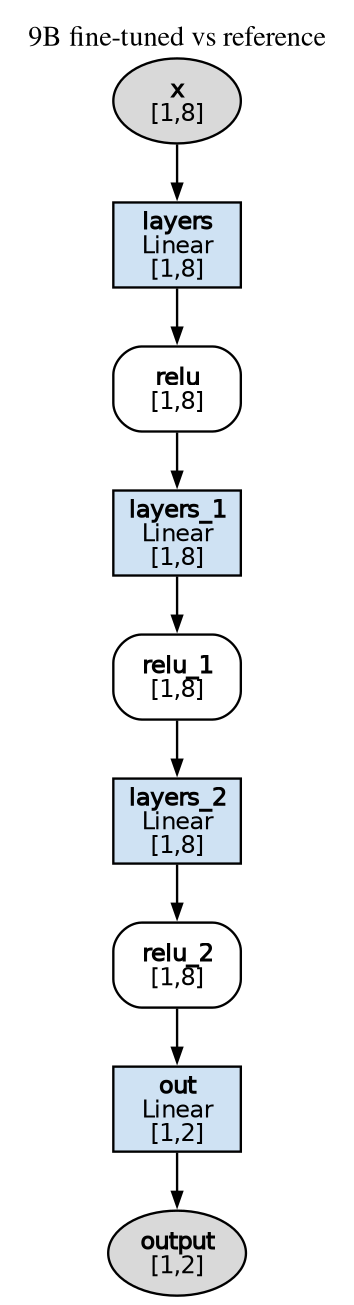
\includegraphics[width=\linewidth,height=0.40\textheight,keepaspectratio]{figs/ex08_ft9b_c_diff.png}\\\footnotesize 9B fine-tuned vs reference\end{minipage}\hfill
\begin{minipage}[b]{0.32\linewidth}\centering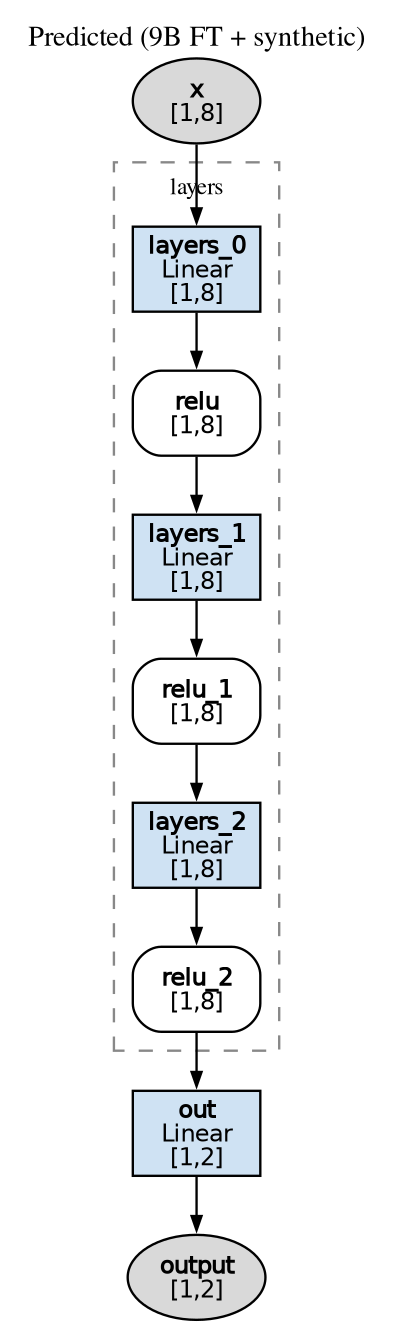
\includegraphics[width=\linewidth,height=0.40\textheight,keepaspectratio]{figs/ex08_ft9b_aug_c_pred.png}\\\footnotesize 9B FT + synthetic (exact)\end{minipage}\hfill
\caption{Example 8 (OOD\_modulelist\_1). Diff colours: black = matched, red dashed = missing (reference only), orange = hallucinated (prediction only), red text = wrong kind or shape.}
\end{figure}
\clearpage

\subsection{Example 9: OOD: Squeeze-and-Excitation, fixed by verify-and-retry}\label{sec:ex09}
{\small set: OOD-1 \textbullet{} sample: \texttt{OOD\_se\_1} \textbullet{} category: \texttt{squeeze\_excite} \textbullet{} 12 nodes}

\lstinputlisting[style=py]{code/ex09.py}
\begin{center}\footnotesize\begin{tabular}{lcccccp{4.6cm}}\toprule
model & valid & edge F1 & exact & shape acc. & tokens & failure labels \\ \midrule
9B FT, before/after retry & yes & 0.87 & no & 0.91 & 635 & \raggedright missing edge, extra edge, missing node \tabularnewline
\bottomrule\end{tabular}\end{center}
\textbf{What to look at.} \emph{Verify-and-retry}: the validator's messages (which never use the reference)
are sent back to the model as a new chat turn. The first attempt left the output node disconnected
(\texttt{output node needs >=1 input}, \texttt{node 0 'x' does not lead to the output}). After one retry round the graph
passes every validity check, but it is \emph{still not exactly right} (edge F1 0.87, one node missing): a valid graph
is not necessarily a correct graph. Over OOD-1, retry raised the fine-tuned 9B from 47.5\% to 67.5\% valid and from
30\% to 45\% exact.

\begin{figure}[H]\centering
\begin{minipage}[b]{0.32\linewidth}\centering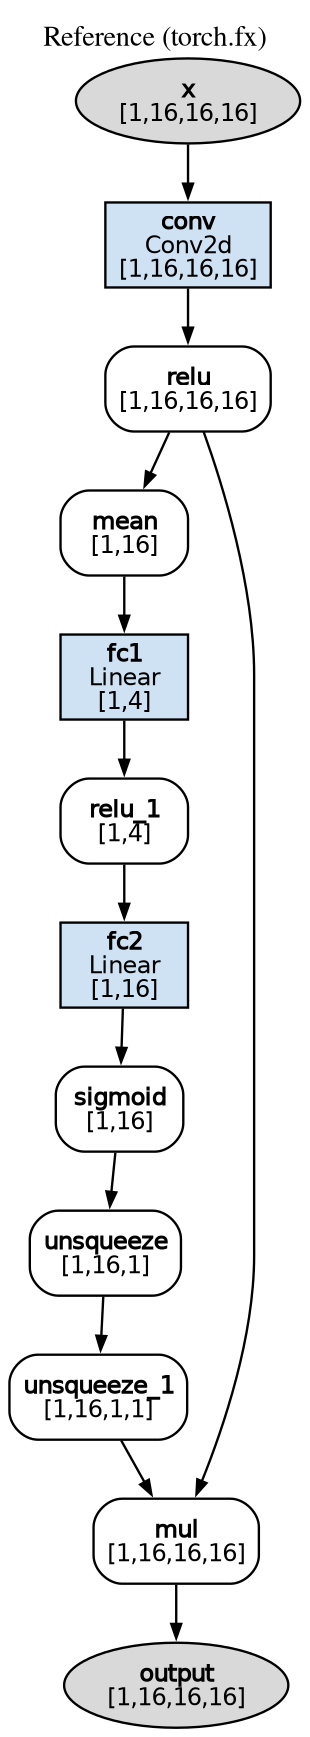
\includegraphics[width=\linewidth,height=0.40\textheight,keepaspectratio]{figs/ex09_ref.png}\\\footnotesize Reference\end{minipage}\hfill
\begin{minipage}[b]{0.32\linewidth}\centering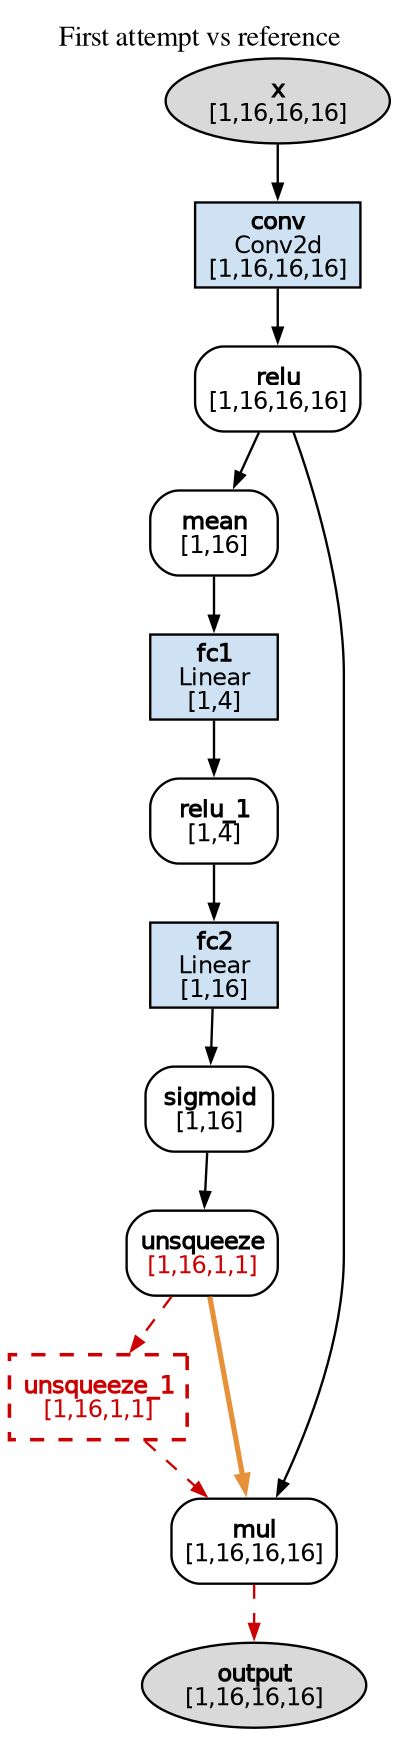
\includegraphics[width=\linewidth,height=0.40\textheight,keepaspectratio]{figs/ex09_ft9b_c_retry_initial_diff.png}\\\footnotesize first attempt vs reference\end{minipage}\hfill
\begin{minipage}[b]{0.32\linewidth}\centering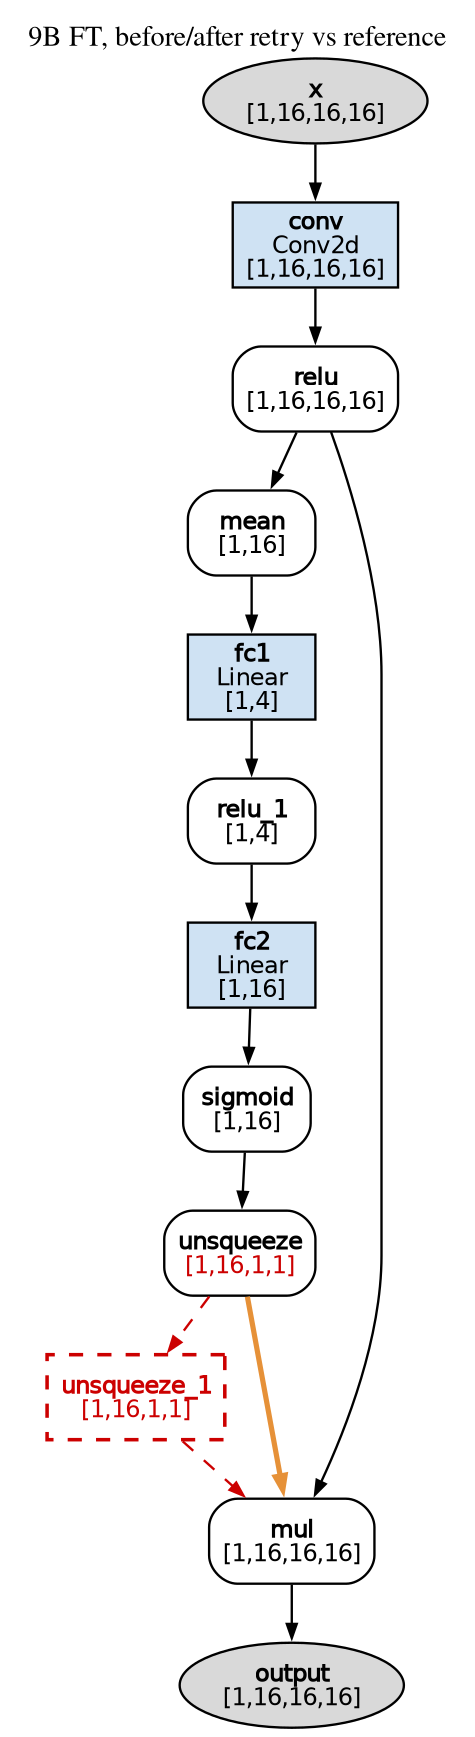
\includegraphics[width=\linewidth,height=0.40\textheight,keepaspectratio]{figs/ex09_ft9b_c_retry_diff.png}\\\footnotesize after 1 retry round\end{minipage}\hfill
\caption{Example 9 (OOD\_se\_1). Diff colours: black = matched, red dashed = missing (reference only), orange = hallucinated (prediction only), red text = wrong kind or shape.}
\end{figure}
\clearpage

\subsection{Example 10: OOD-2: a transposed-convolution decoder (shape failure)}\label{sec:ex10}
{\small set: OOD-2 \textbullet{} sample: \texttt{OOD2\_deconv\_2} \textbullet{} category: \texttt{transposed\_conv} \textbullet{} 9 nodes}

\lstinputlisting[style=py]{code/ex10.py}
\begin{center}\footnotesize\begin{tabular}{lcccccp{4.6cm}}\toprule
model & valid & edge F1 & exact & shape acc. & tokens & failure labels \\ \midrule
9B FT + synthetic & no & 1.00 & yes & 0.11 & 291 & \raggedright shape only \tabularnewline
27B 3-shot & yes & 1.00 & yes & 1.00 & 281 & \raggedright -- \tabularnewline
\bottomrule\end{tabular}\end{center}
\textbf{What to look at.} OOD-2 deliberately uses operators that appear in neither the dataset nor the
synthetic generator, here \texttt{nn.ConvTranspose2d} (an up-sampling convolution). The synthetic-data 9B gets the
\emph{topology} exactly right (all edges black) but almost all \emph{shapes} wrong (red shape text, shape accuracy
11\%). The mistake starts at the very first layer: the model ignores the \texttt{stride=2} of the ordinary
convolution \texttt{down} and predicts \texttt{[1,8,16,16]} instead of \texttt{[1,8,8,8]}. Every later shape inherits
the error, so the transposed convolution then ``doubles'' 16 to 32 instead of 8 to 16. The shape check catches the
inconsistency at the final skip addition (\texttt{add\_1 inputs [1,4,16,16] and [1,4,32,32] are not
broadcast-compatible}). The 27B model gets
this one fully right. Shape propagation through unseen operators is the main remaining weakness of all fine-tuned
models.

\begin{figure}[H]\centering
\begin{minipage}[b]{0.47\linewidth}\centering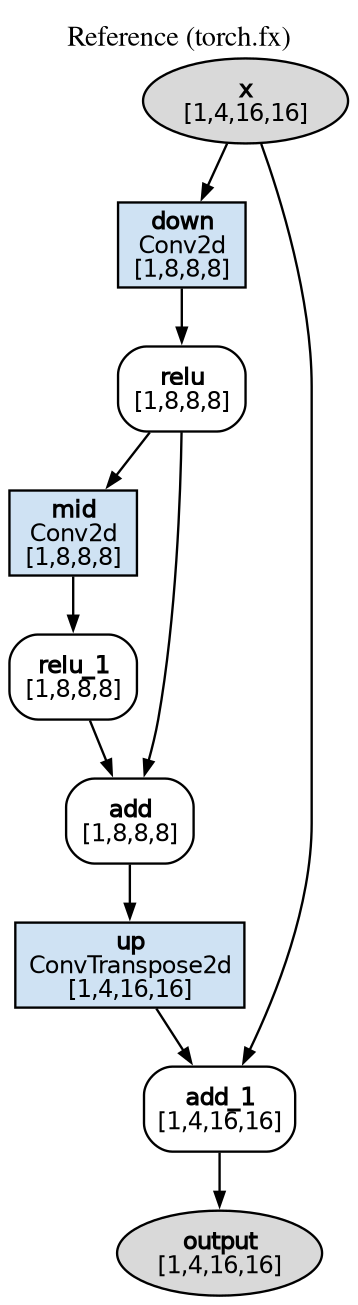
\includegraphics[width=\linewidth,height=0.40\textheight,keepaspectratio]{figs/ex10_ref.png}\\\footnotesize Reference\end{minipage}\hfill
\begin{minipage}[b]{0.47\linewidth}\centering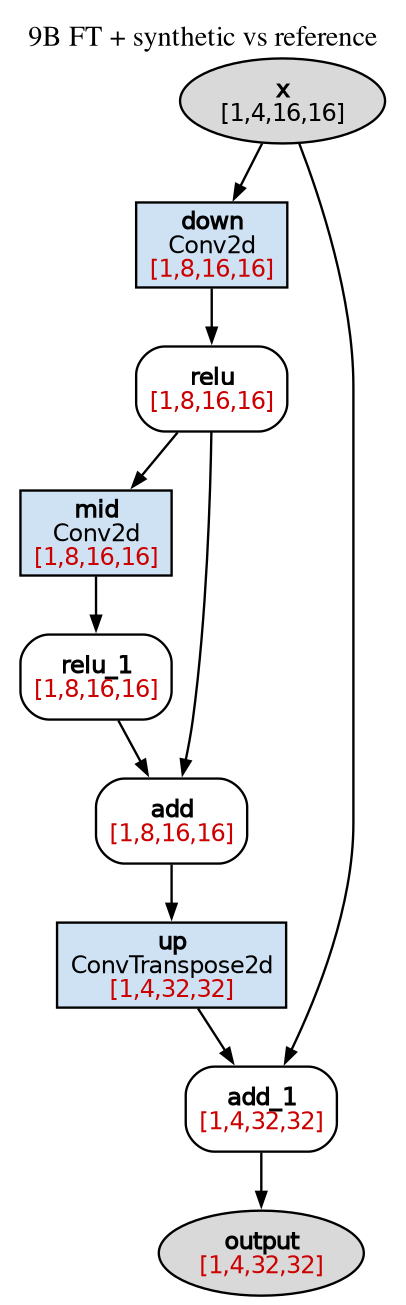
\includegraphics[width=\linewidth,height=0.40\textheight,keepaspectratio]{figs/ex10_ft9b_aug_c_diff.png}\\\footnotesize 9B FT + synthetic vs reference\end{minipage}\hfill
\caption{Example 10 (OOD2\_deconv\_2). Diff colours: black = matched, red dashed = missing (reference only), orange = hallucinated (prediction only), red text = wrong kind or shape.}
\end{figure}
\clearpage

\subsection{Example 11: OOD-2: attention with matmul and softmax}\label{sec:ex11}
{\small set: OOD-2 \textbullet{} sample: \texttt{OOD2\_attn\_1} \textbullet{} category: \texttt{matmul\_attention} \textbullet{} 13 nodes}

\lstinputlisting[style=py]{code/ex11.py}
\begin{center}\footnotesize\begin{tabular}{lcccccp{4.6cm}}\toprule
model & valid & edge F1 & exact & shape acc. & tokens & failure labels \\ \midrule
9B FT + synthetic & yes & 1.00 & yes & 1.00 & 349 & \raggedright -- \tabularnewline
27B 3-shot & no & 1.00 & yes & 0.69 & 355 & \raggedright shape only \tabularnewline
\bottomrule\end{tabular}\end{center}
\textbf{What to look at.} A tiny attention block (\texttt{unsqueeze}, \texttt{matmul}, \texttt{softmax},
\texttt{squeeze}; method calls become \texttt{call\_method} nodes). Here the roles flip: the synthetic-data 9B is
exactly right, while the 27B gets the topology right but adds an edge to a node index that does not exist and gets 31\%
of the shapes wrong, so the validator rejects it. Bigger is better on average, not on every example.

\begin{figure}[H]\centering
\begin{minipage}[b]{0.32\linewidth}\centering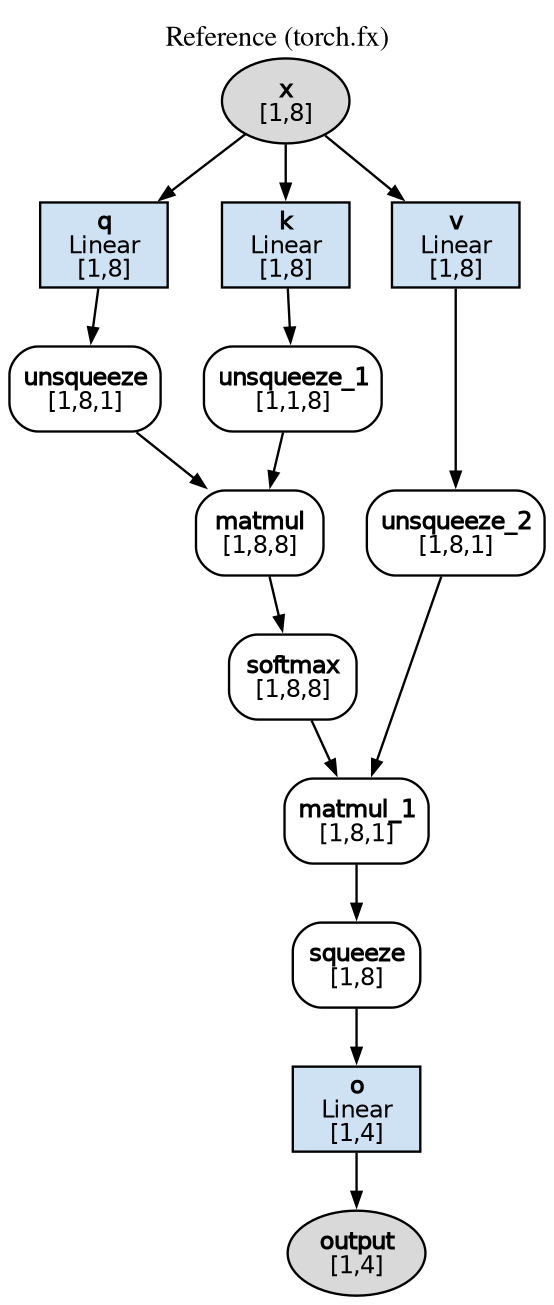
\includegraphics[width=\linewidth,height=0.40\textheight,keepaspectratio]{figs/ex11_ref.png}\\\footnotesize Reference\end{minipage}\hfill
\begin{minipage}[b]{0.32\linewidth}\centering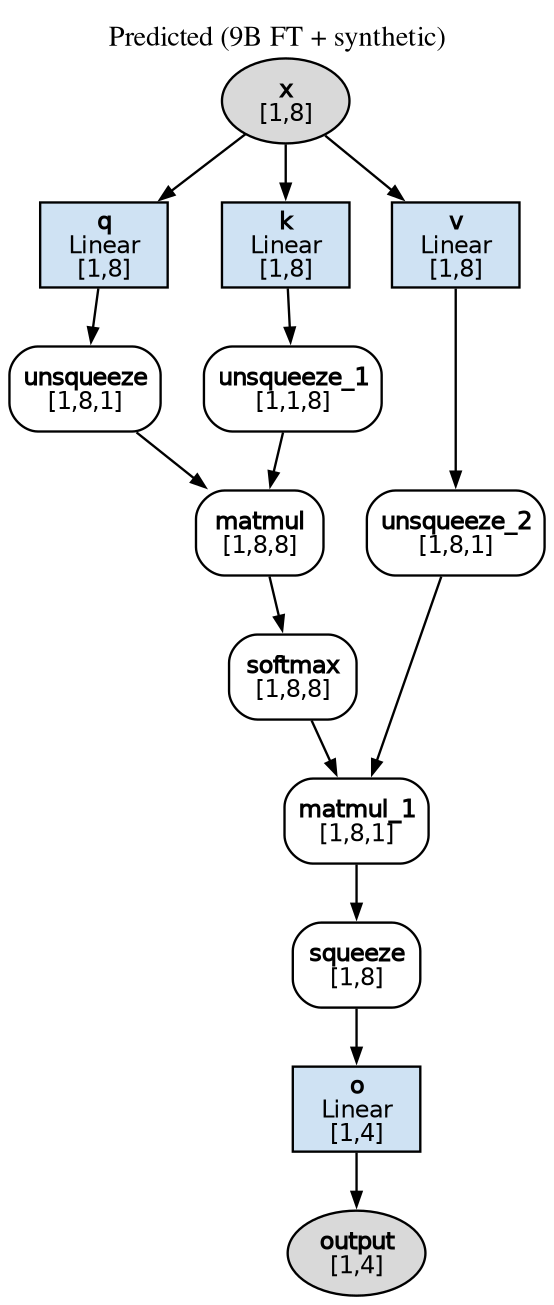
\includegraphics[width=\linewidth,height=0.40\textheight,keepaspectratio]{figs/ex11_ft9b_aug_c_pred.png}\\\footnotesize 9B FT + synthetic (exact)\end{minipage}\hfill
\begin{minipage}[b]{0.32\linewidth}\centering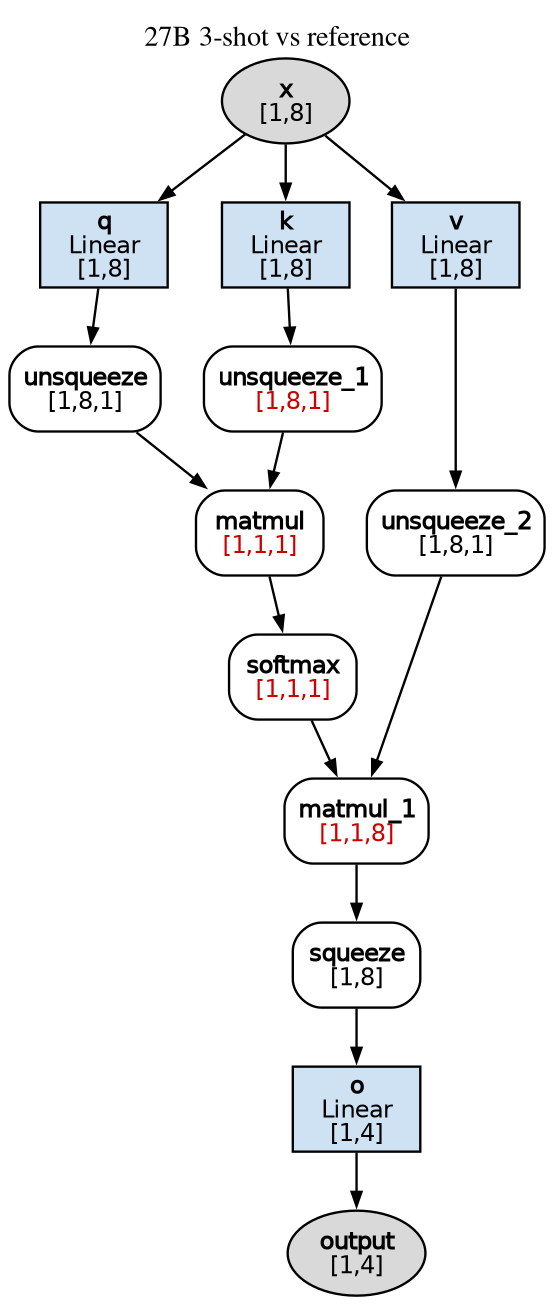
\includegraphics[width=\linewidth,height=0.40\textheight,keepaspectratio]{figs/ex11_ceil_fs_c_diff.png}\\\footnotesize 27B 3-shot vs reference\end{minipage}\hfill
\caption{Example 11 (OOD2\_attn\_1). Diff colours: black = matched, red dashed = missing (reference only), orange = hallucinated (prediction only), red text = wrong kind or shape.}
\end{figure}
\clearpage

\subsection{Example 12: Untraceable code: no torch.fx reference exists}\label{sec:ex12}
{\small set: untraceable set \textbullet{} sample: \texttt{UNT\_data\_dependent\_if} \textbullet{} category: \texttt{untraceable}}

\lstinputlisting[style=py]{code/ex12.py}
\begin{center}\footnotesize\begin{tabular}{lcccccp{4.6cm}}\toprule
model & valid & edge F1 & exact & shape acc. & tokens & failure labels \\ \midrule
9B fine-tuned & no & -- & n/a & -- & 160 & \raggedright n/a \tabularnewline
\bottomrule\end{tabular}\end{center}
\textbf{What to look at.} The \texttt{if} depends on the \emph{value} of the input, so
\texttt{torch.fx.symbolic\_trace} raises \texttt{TraceError}: there is no reference graph, and this is exactly where an
LLM can still be useful. The fine-tuned 9B draws both branches feeding the output (it cannot know which branch runs),
which the validator reports as \texttt{output node has 2 inputs}. The validator also wrongly reports \texttt{conv} as
dead code: its code analysis only follows straight-line code and does not look inside \texttt{if} bodies (a known
limitation, Section~\ref{sec:caveats}). These examples are qualitative only.

\begin{figure}[H]\centering
\begin{minipage}[b]{0.55\linewidth}\centering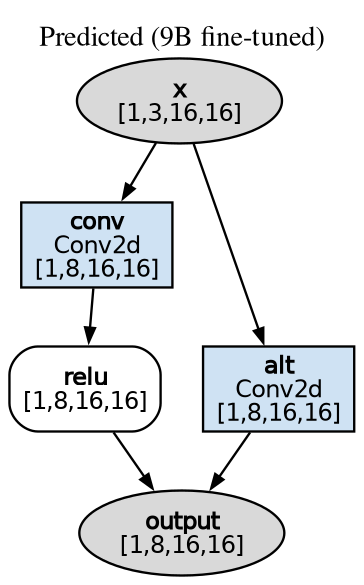
\includegraphics[width=\linewidth,height=0.36\textheight,keepaspectratio]{figs/ex12_ft9b_c_pred.png}\\\footnotesize 9B fine-tuned prediction (no reference exists)\end{minipage}\hfill
\caption{Example 12 (UNT\_data\_dependent\_if). Diff colours: black = matched, red dashed = missing (reference only), orange = hallucinated (prediction only), red text = wrong kind or shape.}
\end{figure}
\clearpage
